\let\lesson\undefined
\newcommand{\lesson}{\phantomlesson{Bài 7.}}
\setcounter{section}{2}
\section{Bài tập trắc nghiệm}

\begin{enumerate}[label=\bfseries Câu \arabic*:]
	
	\item \mkstar{2}\\
	{Chuyển động thẳng chậm dần đều có
		\begin{mcq}
			\item quỹ đạo là đường cong bất kì.
			\item độ lớn vectơ gia tốc là một hằng số, ngược chiều với vectơ vận tốc của vật.
			\item quãng đường đi được của vật không phụ thuộc vào thời gian.
			\item vectơ vận tốc vuông góc với quỹ đạo của chuyển động.
		\end{mcq}
	
}
\hideall{
\textbf{Đáp án: B.}
}

\item \mkstar{2}\\
{Chọn phát biểu đúng.
	\begin{mcq}
		\item Gia tốc của chuyển động thẳng nhanh dần đều bao giờ cũng lớn hơn gia tốc của chuyển động thẳng chậm dần đều.
		\item Chuyển động thẳng nhanh dần đều có gia tốc lớn thì có vận tốc lớn.
		\item Chuyển động thẳng biến đổi đều có gia tốc tăng, giảm đều theo thời gian.
		\item Gia tốc trong chuyển động thẳng nhanh dần đều có phương, chiều và độ lớn không đổi.
	\end{mcq}

}
\hideall{
\textbf{Đáp án: D.}
}

\item \mkstar{2}\\
{Gọi $v_0$ là vận tốc ban đầu của chuyển động. Công thức liên hệ giữa vận tốc $v$, gia tốc $a$ và quãng đường $s$ vật đi được trong chuyển động thẳng biến đổi đều là
\begin{mcq}(4)
	\item $v+v_0=\sqrt{2as}$.
	\item $v-v_0=\sqrt{2as}$.
	\item $v^2+v^2_0=2as$.
	\item $v^2-v^2_0=2as$.
\end{mcq}
}
\hideall{
\textbf{Đáp án: D.}
}
\item \mkstar{2}\\
{Công thức tính quãng đường đi được của chuyển động thẳng nhanh dần đều là
\begin{mcq}(2)
	\item $s=v_0t+\dfrac{1}{2}at^2$ ($a$ và $v_0$ cùng dấu).
	\item $s=v_0t+\dfrac{1}{2}at^2$ ($a$ và $v_0$ trái dấu).
	\item $x=x_0+v_0t+\dfrac{1}{2}at^2$ ($a$ và $v_0$ cùng dấu).
	\item $x=x_0+v_0t+\dfrac{1}{2}at^2$ ($a$ và $v_0$ trái dấu).
\end{mcq}
}
\hideall{
\textbf{Đáp án: A.}
}

\item \mkstar{2}\\
{Trong công thức tính vận tốc của chuyển động thẳng nhanh dần đều $v = v_0 + at$, thì
\begin{mcq}(2)
	\item $v$ luôn dương.
	\item $a$ luôn dương.
	\item tích $a\cdot v$ luôn dương.
	\item tích $a\cdot v$ luôn âm.
\end{mcq}
}
\hideall{
\textbf{Đáp án: C.}
}

	\item \mkstar{2}\\
	{\begin{minipage}[l]{0.7\textwidth}
			Một vật chuyển động thẳng biến đổi đều mà vận tốc được biểu diễn bởi đồ thị như hình vẽ.\\
			Chuyển động của vật là chuyển động chậm dần đều vì
			\begin{mcq}
				\item đường biểu diễn của vận tốc là đường thẳng.
				\item độ lớn vận tốc tăng theo thời gian.
				\item độ lớn vận tốc giảm đều theo thời gian.
				\item độ lớn vận tốc là hàm bậc nhất theo thời gian.
			\end{mcq}
		\end{minipage}
	\begin{minipage}{0.3\textwidth}
		\begin{center}
			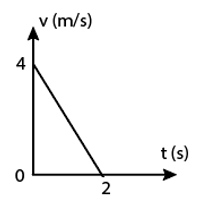
\includegraphics[width=0.8\linewidth]{../figs/VN10-2023-PH-TP009-P-1}
		\end{center}
	\end{minipage}
Gia tốc của chuyển động là
\begin{mcq}(4)
	\item $\SI{-2}{\meter/\second^2}$.
	\item $\SI{2}{\meter/\second^2}$.
	\item $\SI{4}{\meter/\second^2}$.
	\item$\SI{-4}{\meter/\second^2}$.
\end{mcq}
Quãng đường mà vật đi được trong $\SI{2}{\second}$ là 
\begin{mcq}(4)
	\item $\SI{1}{\meter}$.
	\item $\SI{4}{\meter}$.
	\item $\SI{6}{\meter}$.
	\item $\SI{8}{\meter}$.
\end{mcq}
}
\hideall{
\textbf{Đáp án: C - A - B.}
}

\item \mkstar{2}\\
{Phương trình nào sau đây là phương trình tọa độ của một vật chuyển động thẳng chậm dần đều dọc theo trục $Ox$?
	\begin{mcq}(2)
		\item $s=2t-3t^2$.
		\item $x=5t^2-2t+5$.
		\item $v=4-t$.
		\item $x=2-5t-t^2$.
	\end{mcq}

}
\hideall{
\textbf{Đáp án: B.}
}

\item \mkstar{3}\\
{Một ô tô chuyển động thẳng biến đổi đều từ trạng thái nghỉ, đạt vận tốc $\SI{20}{\meter/\second}$ sau $\SI{5}{\second}$. Quãng đường mà ô tô đã đi được là
\begin{mcq}(4)
	\item $\SI{100}{\meter}$.
	\item $\SI{50}{\meter}$.
	\item $\SI{25}{\meter}$.
	\item $\SI{200}{\meter}$.
\end{mcq}
}
\hideall{
\textbf{Đáp án: B.}
}

\item \mkstar{3}\\
{Xe ô tô đang chuyển động thẳng với vận tốc $\SI{20}{\meter/\second}$ thì bị hãm phanh chuyển động chậm dần đều. Quãng đường xe đi được từ lúc hãm phanh đến khi xe dừng hẳn là $\SI{100}{\meter}$. Gia tốc của xe là
\begin{mcq}(4)
	\item $\SI{1}{\meter/\second^2}$.
	\item $\SI{-1}{\meter/\second^2}$.
	\item $\SI{-2}{\meter/\second^2}$.
	\item $\SI{5}{\meter/\second^2}$.
\end{mcq}
}
\hideall{
\textbf{Đáp án: C.}
}

\item \mkstar{3}\\
{Một ô tô chuyển động chậm dần đều. Sau $\SI{10}{\second}$ vận tốc của ô tô giảm từ $\SI{6}{\meter/\second}$ về $\SI{4}{\meter/\second}$. Quãng đường ô tô đi được trong khoảng thời gian $\SI{10}{\second}$ đó là
	\begin{mcq}(4)
		\item $\SI{70}{\meter}$.
		\item $\SI{50}{\meter}$.
		\item $\SI{40}{\meter}$.
		\item $\SI{100}{\meter}$.
	\end{mcq}

}
\hideall{
\textbf{Đáp án: B.}
}

\item \mkstar{3}\\
{Một ô tô đang chuyển động với vận tốc $\SI{10}{\meter/\second}$ thì bắt đầu tăng ga (tăng tốc), chuyển động nhanh dần đều. Sau $\SI{20}{\second}$ ô tô đạt được vận tốc $\SI{14}{\meter/\second}$. Sau $\SI{50}{\second}$ kể từ lúc tăng tốc, gia tốc và vận tốc của ô tô lần lượt là
\begin{mcq}(4)
	\item $a=\SI{0.2}{\meter/\second^2}$ và $\SI{18}{\meter/\second}$.
	\item $a=\SI{0.2}{\meter/\second^2}$ và $\SI{20}{\meter/\second}$.
	\item $a=\SI{0.4}{\meter/\second^2}$ và $\SI{38}{\meter/\second}$.
	\item $a=\SI{0.1}{\meter/\second^2}$ và $\SI{28}{\meter/\second}$.
\end{mcq}
}
\hideall{
\textbf{Đáp án: B.}
}

\item \mkstar{3}\\
{Tàu hỏa đang chuyển động với vận tốc $\SI{60}{\kilo\meter/\hour}$ thì bị hãm phanh chuyển động chậm dần đều. Sau khi đi thêm được $\SI{450}{\meter}$ thì vận tốc của tàu chỉ còn $\SI{15}{\kilo\meter/\hour}$. Quãng đường tàu còn đi thêm được đến khi dừng hẳn là
\begin{mcq}(4)
	\item $\SI{60}{\meter}$.
	\item $\SI{45}{\meter}$.
	\item $\SI{15}{\meter}$.
	\item $\SI{30}{\meter}$.
\end{mcq}
}
\hideall{
\textbf{Đáp án: D.}
}
	\item \mkstar{3}\\
	{\begin{minipage}[l]{0.7\textwidth}
			Đồ thị vận tốc - thời gian của một tàu hỏa đang chuyển động thẳng có dạng như hình bên. Thời điểm $t = 0$ là lúc tàu đi qua sân ga. Vận tốc của tàu sau khi rời sân ga được $\SI{80}{\meter}$ là
			\begin{mcq}(2)
				\item $\SI{4}{\meter/\second}$.
				\item $\SI{6}{\meter/\second}$.
				\item $\SI{8}{\meter/\second}$.
				\item $\SI{10}{\meter/\second}$.
			\end{mcq}
		\end{minipage}
		\begin{minipage}{0.3\textwidth}
			\begin{center}
				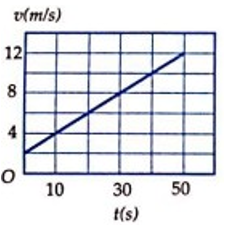
\includegraphics[width=0.6\linewidth]{../figs/VN10-2022-PH-TP008-P-3}
			\end{center}
		\end{minipage}
	}
	\hideall{
		\textbf{Đáp án: B.}
	}

\item \mkstar{3}\\
{\begin{minipage}[l]{0.7\textwidth}
Một vật chuyển động thẳng biến đổi đều có đồ thị vận tốc $v$ theo thời gian $t$ như hình vẽ. Phương trình vận tốc của vật là
		\begin{mcq}(2)
			\item $v=15-t \left(\si{\meter/\second}\right)$.
			\item $v=15+t \left(\si{\meter/\second}\right)$.
			\item $v=10-5t \left(\si{\meter/\second}\right)$.
			\item $v=10-5t \left(\si{\meter/\second}\right)$.
		\end{mcq}
	\end{minipage}
	\begin{minipage}{0.3\textwidth}
		\begin{center}
			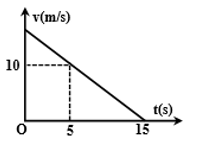
\includegraphics[width=0.8\linewidth]{../figs/VN10-2023-PH-TP009-P-2}
		\end{center}
	\end{minipage}
}
\hideall{
\textbf{Đáp án: A.}
}

\item \mkstar{3}\\
{\begin{minipage}[l]{0.7\textwidth}
		Một vật chuyển động có đồ thị vận tốc - thời gian như hình vẽ. Quãng đường đi được trong giai đoạn chuyển động thẳng chậm dần đều là
		\begin{mcq}
			\item $\SI{62.5}{\meter}$.
			\item $\SI{75}{\meter}$.
			\item $\SI{37.5}{\meter}$.
			\item $\SI{100}{\meter}$.
		\end{mcq}
	\end{minipage}
\begin{minipage}{0.3\textwidth}
	\begin{center}
		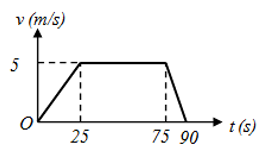
\includegraphics[width=0.8\linewidth]{../figs/VN10-2023-PH-TP009-P-3}
	\end{center}
\end{minipage}
}
\hideall{
\textbf{Đáp án: C.}
}

\item \mkstar{3}\\
{Phương trình của một vật chuyển động thẳng biến đổi đều là: $x = 20t^2 + 40t + 6$ (cm; s). Tính gia tốc và tính chất của chuyển động.
	\begin{mcq}(2)
		\item $\SI{40}{\centi\meter/\second^2}$; vật chuyển động nhanh dần đều.
		\item $\SI{40}{\centi\meter/\second^2}$; vật chuyển động chậm dần đều.
		\item $\SI{20}{\centi\meter/\second^2}$; vật chuyển động nhanh dần đều.
		\item $\SI{20}{\centi\meter/\second^2}$; vật chuyển động chậm dần đều.
	\end{mcq}

}
\hideall{
\textbf{Đáp án: A.}
}

\item \mkstar{3}\\
{Một vật chuyển động trên đường thẳng theo phương trình: $x=-t^2+2t$ $\left(\si{\meter}, \si{\second}\right)$. Tốc độ trung bình từ thời điểm $t_1 = \SI{0.75}{\second}$ đến $t_2 = \SI{3}{\second}$ bằng
	\begin{mcq}(4)
		\item $\SI{3.6}{\meter/\second}$.
		\item $\SI{9.2}{\meter/\second}$.
		\item $\SI{2.7}{\meter/\second}$.
		\item $\SI{1.8}{\meter/\second}$.
	\end{mcq}

}
\hideall{
\textbf{Đáp án: D.}
}

\item \mkstar{4}\\
{Một xe chuyển động nhanh dần đều với vận tốc đầu $\SI{18}{\kilo\meter/\hour}$. Trong giây thứ 5 xe đi được $\SI{14}{\meter}$. \\
	Gia tốc của xe là
	\begin{mcq}(4)
		\item $\SI{4}{\meter/\second^2}$.
		\item $\SI{3}{\meter/\second^2}$.
		\item $\SI{2}{\meter/\second^2}$.
		\item $\SI{6}{\meter/\second^2}$.
	\end{mcq}
Quãng đường đi được trong giây thứ 10
\begin{mcq}(4)
	\item $\SI{24}{\meter}$.
	\item $\SI{34}{\meter}$.
	\item $\SI{14}{\meter}$.
	\item $\SI{44}{\meter}$.
\end{mcq}
}
\hideall{
\textbf{Đáp án: C - A.}
}
\end{enumerate}
\section{Bài tập tự luận}
\begin{enumerate}[label=\bfseries Bài \arabic*:]
	\item \mkstar{3}
	
	{ Từ các đồ thị trong hình:
		\begin{center}
			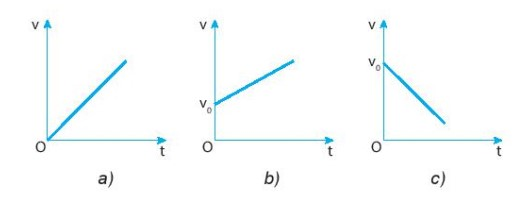
\includegraphics[scale=1]{../figs/VN10-2022-PH-TP012-1.jpg}
		\end{center}
		
		\begin{enumerate}[label=\alph*)]
			\item Hãy viết công thức về mối liên hệ giữa $v$ với $a$ và $t$ của từng chuyển động ứng với từng đồ thị trong hình.
			\item Chuyển động nào là chuyển động nhanh dần dều, chậm dần đều?
		\end{enumerate}
		
	}
	
	\hideall{
		
		\begin{enumerate}[label=\alph*)]
			\item 
			- Đồ thị a: $$v=at.$$
			
			- Đồ thị b: $$v = v_0 + at.$$
			
			- Đồ thị c: $$v = v_0 -at.$$
			\item 
			
			- Chuyển động nhanh dần đều là: đồ thị a và b.
			
			- Chuyển động chậm dần đều: đồ thị c.
			
			
			
			
		\end{enumerate}
		
	}

		\item \mkstar{2}
	
	{
		Một ô tô tăng tốc từ lúc đứng yên, sau $\SI{6}{s}$ đạt vận tốc $\SI{18}{m/s}$. Tính độ lớn gia tốc của ô tô.
	}
	\hideall{
		
		Gia tốc của ô tô
		
		$$a = \dfrac{v_2 - v_1}{t} = \dfrac{18 - 0}{6} = \SI{3}{m/s}^2.$$
	}
	\item \mkstar{2}
	
	{
		Người lái xe ô tô hãm phanh để xe giảm tốc độ từ $\SI{23}{m/s}$ đến $\SI{11}{m/s}$ trong $\SI{20}{s}$. Tính độ lớn của gia tốc.
	}
	\hideall{
		
		Độ lớn của gia tốc
		
		$$a = \dfrac{v_2 - v_1}{t} = \dfrac{11-23}{20} = -\SI{0,6}{m/s}^2.$$
	}
	\item \mkstar{2}
	
	{
		Trong một cuộc thi chạy, từ trạng thái đứng yên, một vận động viên chạy với gia tốc $\SI{5}{m/s}^2$ trong 2 giây đầu tiên. Tính vận tốc của vận động viên sau 2 giây.
	}
	\hideall{
		
		Vận tốc của vận động viên
		
		$$a = \dfrac{v_2 - v_1}{t} \Rightarrow v_2 = at = \SI{10}{m/s}.$$
	}
	\item \mkstar{3}
	
	{
		Bảng dưới đây ghi vận tốc tức thời đo bởi tốc kế của một ô tô sau các khoảng thời gian $\SI{2}{s}$ kể từ khi bắt đầu chạy trên một đường thẳng.
		
		\begin{center}
			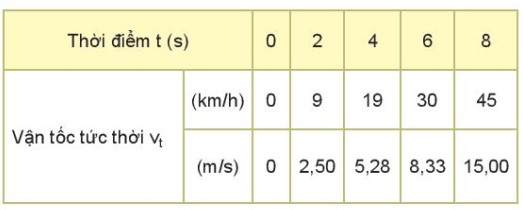
\includegraphics[scale=1]{../figs/VN10-2022-PH-TP007-1.jpg}
		\end{center}
		
		\begin{enumerate}[label=\alph*)]
			\item Xác định độ biến thiên vận tốc sau $\SI{8}{s}$ của chuyển động trên.
			\item Xác định độ biến thiên của vận tốc sau mỗi giây của chuyển động trên trong $\SI{4}{s}$ đầu và trong $\SI{4}{s}$ cuối.
		\end{enumerate}
	}
	\hideall{
		
		\begin{enumerate}[label=\alph*)]
			\item 
			Độ biến thiên vận tốc sau 8 giây là
			
			$$\Delta v = v_8 - v_0 = \SI{45}{km/h}.$$
			\item Độ biến thiên vận tốc trong 4 giây đầu là
			
			$$\Delta v = v_4 - v_0 = \SI{5,28}{m/s}.$$
			
			Độ biến thiên của vận tốc sau mỗi giây của chuyển động trên trong 4 giây đầu là :
			
			$$\dfrac{\Delta v}{\Delta t} = \SI{1,32}{m/s}^.$$
			
			Độ biến thiên vận tốc trong 4 giây sau là: 
			
			$$\Delta v' = v_8 - v_4 =\SI{7,22}{m/s}.$$
			
			Độ biến thiên của vận tốc sau mỗi giây của chuyển động trên trong 4 giây sau là:
			
			$$\dfrac{\Delta v'}{\Delta t} = \SI{1,805}{m/s}^2.$$ 
		\end{enumerate}
	}
	\item \mkstar{3}
	
	{
		Một xe máy đang chuyển động thẳng với vận tốc $\SI{10}{m/s}$ thì tăng tốc. Sau $\SI{5}{s}$ đạt vận tốc $\SI{12}{m/s}.$
		
		\begin{enumerate}[label=\alph*)]
			\item Tính gia tốc của xe.
			\item Nếu sau khi đạt vận tốc $\SI{12}{m/s}$, xe chuyển động chậm dần với gia tốc có độ lớn bằng gia tốc trên thì sau bao lâu xe dừng lại?
		\end{enumerate}
	}
	\hideall{
		
		\begin{enumerate}[label=\alph*)]
			\item Gia tốc của xe
			
			$$a = \dfrac{\Delta v}{\Delta t} = \SI{0,4}{m/s}^2.$$
			
			\item Thời gian xe dừng lại
			
			$$\Delta t' = \dfrac{\Delta v'}{a} = \SI{30}{s}.$$
		\end{enumerate}
		
	}

	\item \mkstar{3}
	
	{
		
		Một con báo đang chạy với vận tốc $\SI{30}{m/s}$ thì chuyển động chậm dần khi tới gần một con suối. Trong 3 giây, vận tốc của nó giảm còn $\SI{9}{m/s}$. Tính gia tốc của con báo.
	}
	\hideall{
		
		Gia tốc của con báo là:
		
		$$a = \dfrac{v_2 - v_1}{t} = - \SI{9}{m/s}^2.$$
	}
	\item \mkstar{3}
	
	{
		
		Đồ thị mô tả sự thay đổi vận tốc theo thời gian trong chuyển động của một ô tô thể thao đang chạy thử về phía Bắc. Tính gia tốc của ô tô:
		\begin{center}
			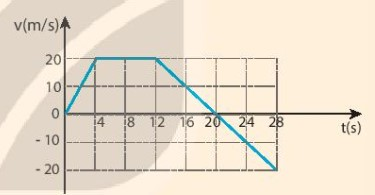
\includegraphics[scale=1]{../figs/VN10-2022-PH-TP007-3.jpg}
		\end{center}
		
		\begin{enumerate}[label=\alph*)]
			\item Trong $\SI{4}{s}$.
			\item Từ giây thứ 4 đến giây thứ 12.
			\item Từ giây thứ 12 đến giây thứ 20.
			\item Từ giây thứ 20 đến giây thứ 28.
		\end{enumerate}
	}
	\hideall{
		
		\begin{enumerate}[label=\alph*)]
			\item Trong $\SI{4}{s}$
			
			$$a_1 = \dfrac{20 -0}{4- 0} = \SI{5}{m/s}^2.$$
			
			\item Từ giây thứ 4 đến giây thứ 12
			
			$$a_2 = \dfrac{20 - 20}{12-4} = \SI{0}{m/s}^2.$$
			
			\item Từ giây thứ 12 đến giây thứ 20
			
			$$a_3 = \dfrac{0 - 20}{20-12} = -\SI{2,5}{m/s}^2.$$
			
			\item Từ giây thứ 20 đến giây thứ 28
			
			$$a_4 = \dfrac{-20 - 0}{28 -20} = -\SI{2,5}{m/s}^2.$$
		\end{enumerate}
	}
	
	\item \mkstar{3}\\
{Một ô tô đang chuyển động thẳng đều với vận tốc $\SI{45}{\kilo\meter/\hour}$ bỗng tăng ga chuyển động nhanh dần đều.
	\begin{enumerate}[label=\alph*.]
		\item Tính gia tốc của xe biết rằng sau $\SI{30}{\second}$ ô tô đạt vận tốc $\SI{72}{\kilo\meter/\hour}$.
		\item Trong quá trình tăng tốc nói trên, vào thời điểm nào kể từ lúc tăng tốc, vận tốc của xe là $\SI{64.8}{\kilo\meter/\hour}$?
	\end{enumerate}
}
\hideall{Đổi đơn vị $\SI{45}{km/h} = \SI{12,5}{m/s};\ \SI{72}{km/h} = \SI{20}{m/s}$.
	
	Chọn chiều dương là chiều chuyển động.
	
	a. Gia tốc của xe là
	$$a = \dfrac{v-v_0}{t} =\dfrac{\SI{20}{\meter/\second}-\SI{12.5}{\meter/\second}}{\SI{30}{\second}}= \SI{0,25}{m/s}^2.$$
	
	b. Đổi đơn vị $\SI{64,8}{km/h} = \SI{18}{m/s}$.
	
	Xe đạt vận tốc $\SI{64,8}{km/h}$ vào thời điểm 
	$$t= \dfrac{v'-v_0}{a}=\dfrac{\SI{18}{\meter/\second}-\SI{12.5}{\meter/\second}}{\SI{0.25}{\meter/\second^{2}}} = \SI{22}{s}.$$
	
}



	\item \mkstar{3}\\
	{Một người đi xe đạp lên dốc dài $\SI{50}{\meter}$. Tốc độ ở dưới chân dốc là $\SI{18}{\kilo\meter/\hour}$ và ở đầu dốc lúc đến nơi là $\SI{3}{\meter/\second}$. Tính gia tốc của chuyển động và thời gian lên dốc. Coi chuyển động trên là chuyển động chậm dần đều.
	
}
	\hideall{
$a\SI{-0.16}{\meter/\second^2}$, $t=\SI{12.5}{\second}$
}
	\item \mkstar{3}
	
	
	{Đồ thị vận tốc - thời gian ở hình mô tả chuyển động của một chú chó con đang chạy trong một ngõ thẳng và hẹp.
		\begin{center}
			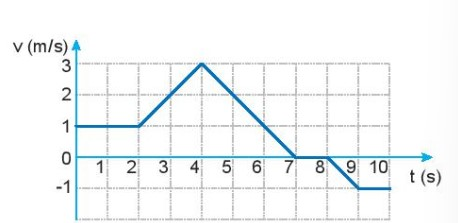
\includegraphics[scale=1]{../figs/VN10-2022-PH-TP012-5.jpg}
		\end{center}
		
		\begin{enumerate}[label=\alph*)]
			\item Hãy mô tả chuyển động của chú chó.
			\item Tính quãng đường đi được và độ dịch chuyển của chú chó sau $\SI{2}{s}$; $\SI{4}{s}$; $\SI{7}{s}$ và $\SI{10}{s}$ bằng đồ thị.
		\end{enumerate}
	}
	
	\hideall
	{	
		\begin{enumerate}[label=\alph*)]
			\item 
			- Trong 2 giây đầu tiên: chuyển động thẳng đều với vận tốc $\SI{1}{m/s}$.
			
			- Từ giây thứ 2 đến giây thứ 4: chuyển động nhanh dần đều.
			
			- Từ giây 4 đến giây 7: chuyển động chậm dần.
			
			- Từ giây 4 đến giây 8: dừng lại.
			
			- Từ giây 8 đến giây 9: chuyển động nhanh dần theo chiều âm.
			
			- Từ giây 9 đến giây 10 chuyển động thẳng đều với vận tốc $-\SI{1}{m/s}$.
			
			
			\item 
			- Sau 2 giây:
			
			$$s_1 = d_1 = v_1 t_1 = \SI{2}{m/s}.$$
			
			- Sau 4 giây:
			
			$$s_2 = d_2 = s_1 + \dfrac{1}{2} (1+3)2 = \SI{6}{m}.$$
			
			- Sau 7 giây:
			
			+ Quãng đường:
			
			$$s_3 = s_2 + \dfrac{1}{2} (7-4)3 = \SI{10,5}{m}.$$
			
			+ Độ dịch chuyển:
			
			$$d_3 = d_2 + \dfrac{1}{2} (7-4)3 = \SI{10,5}{m}.$$
			
			- Sau 10 giây:
			
			+ Quãng đường:
			
			Từ giây 7 – 8: đứng yên
			
			$$s_4 = s_3 + s' = \text{10,5} + \text{0,5} + 1 = \SI{12}{m}.$$
			
			+ Độ dịch chuyển:
			
			$$d_4 = d_3 + d' = \text{10,5} - \text{0,5} - 1 = \SI{9}{m}.$$
			
		\end{enumerate}
	}
	\item \mkstar{4}
	
	
	{Một vận động viên đua xe đạp đường dài vượt qua vạch đích với vận tốc $\SI{10}{m/s}$. Sau đó vận động viên này đi chậm dần đều thêm $\SI{20}{m}$ mới dừng lại. Coi chuyển động của vận động viên là thẳng.
		\begin{enumerate}[label=\alph*)]
			\item Tính gia tốc của vận động viên trong đoạn đường sau khi qua vạch đích.
			\item Tính thời gian vận động viên đó cần để dừng lại kể từ khi cán đích.
			\item Tính tốc độ trung bình của người đó trên quãng đường dừng xe.
		\end{enumerate}
	}
	
	\hideall
	{	
		\begin{enumerate}[label=\alph*)]
			\item Gia tốc của vận động viên trong đoạn đường sau khi qua vạch đích
			
			$$v^2 - v_0^2 = 2ad \Rightarrow a = -\SI{2,5}{m/s}^2.$$
			
			\item Thời gian vận động viên đó cần để dừng lại kể từ khi cán đích
			
			$$a = \dfrac{\Delta v}{\Delta t} \Rightarrow  \Delta t = \SI{4}{s}.$$
			
			\item Tốc độ trung bình của người đó trên quãng đường dừng xe
			
			$$v = \dfrac{d}{t} = \SI{5}{m/s}.$$
		\end{enumerate}
	}
\end{enumerate}
